\documentclass[a4paper]{jpconf}
% \usepackage[square,sort&compress,sectionbib]{natbib}

\usepackage{amsmath}
\usepackage{graphicx}
\usepackage{wrapfig}
\usepackage{cite}
\usepackage{placeins}
\usepackage[table,xcdraw]{xcolor}


% define color
\definecolor{olivegreen}{RGB}{34,139,34}
\definecolor{darkorange}{RGB}{255,140,0}

\begin{document}
\title{Preliminary indirect measurement of cosmic-ray proton spectrum using Earth's $\gamma$-ray data from {\it Fermi} Large Area Telescope}

\author{Patomporn Payoungkhamdee}
\address{Department of Physics, Faculty of Science, Mahidol University, Bangkok 10400, Thailand}
% \address{Production Editor, \jpcs, \iopp, Dirac House, Temple Back, Bristol BS1~6BE, UK}

\ead{patomporn.pay@gmail.com}

\begin{abstract}
Cosmic rays (CRs) are high-energy particles, mostly protons, propagating in space. The rigidity (momentum per charge) spectrum of CRs is well described by a power law for which the spectral index is approximately 2.8 around 30 - 1000 GV. Recent measurements by PAMELA and AMS-02 indicate an abrupt change of the CR proton spectral index at about 340 GV. When CRs interact with the Earth's upper atmosphere, $\gamma$ rays can be produced and detected by space-based detectors. Here we use the Earth's $\gamma$-ray data collected by the {\it Fermi} Large Area Telescope along with a proton-air interaction model to indirectly determine the CR proton spectral index and compare against observations by other instruments.
\end{abstract}

\section{Introduction}
Cosmic-ray are high energy particle which mainly come from the outer space which can penetrate and interact with the Earth's atmosphere \cite{HESS,Pacini,Clay}.
The shark peak of gamma-ray emission from Earth's limb are mainly come from the interaction of CRs with the atmospheric molecules \cite{Warit2009}.

There are many possible phenomena of acceleration mechanism in the
space that could produce high energy particles. The characteristic of acceleration mechanism could roughly be distinguished by a spectral index in the arrival of cosmic rays spectrum in rigidity.
The breaking point of the spectrum mainly come from the overlapped region of acceleration mechanism that could be an evidence to explore a new candidate of cosmic ray source.

In 2011, PAMELA detector indicated that there is a breakpoint of cosmic-ray protons spectrum around 240 GV \cite{PAMELA}.
Furthermore, AMS-02 also found a drastic change of cosmic-ray proton spectrum at around 336 GV \cite{AMS-02}.
From the previous work, 5 years of \textit{Fermi} Large Area Telescope
(\textit{Fermi}-LAT) observation data has been analyzed to trace back
the characteristic of CR proton spectrum where the result imply that there is
a breaking of spectral indice around 200 GeV where the statistical significance
is around 2$\sigma$ \cite{previouswork}. In this work, 9 years of \textit{Fermi}-LAT
data would be use for finding the spectral indices of CR proton between energy
hundred MeV to a TeV range.

\section{Methodology}
\subsection{Data selection and $\gamma$-ray flux extraction}

We use $\sim9$ years (7 Aug 2008 - 16 Oct 2017) of the latest version
(P8R2 ULTRACLEANVETO V6) of the LAT's photon data between 10 GeV to 1 TeV.
We observe $\gamma$ rays from the Earth's thin upper atmosphere by selecting the
nadir angle ($\theta_{\rm NADIR}$) from $68.4^\circ$ to $70.0^\circ$ \cite{previouswork} as
demonstrated in Figure~\ref{gamma_production_schematic}. The incidence angle cut,
$\theta_{\rm LAT}<70^\circ$, is also applied.


% \begin{figure}[h!]
%     \centering
%     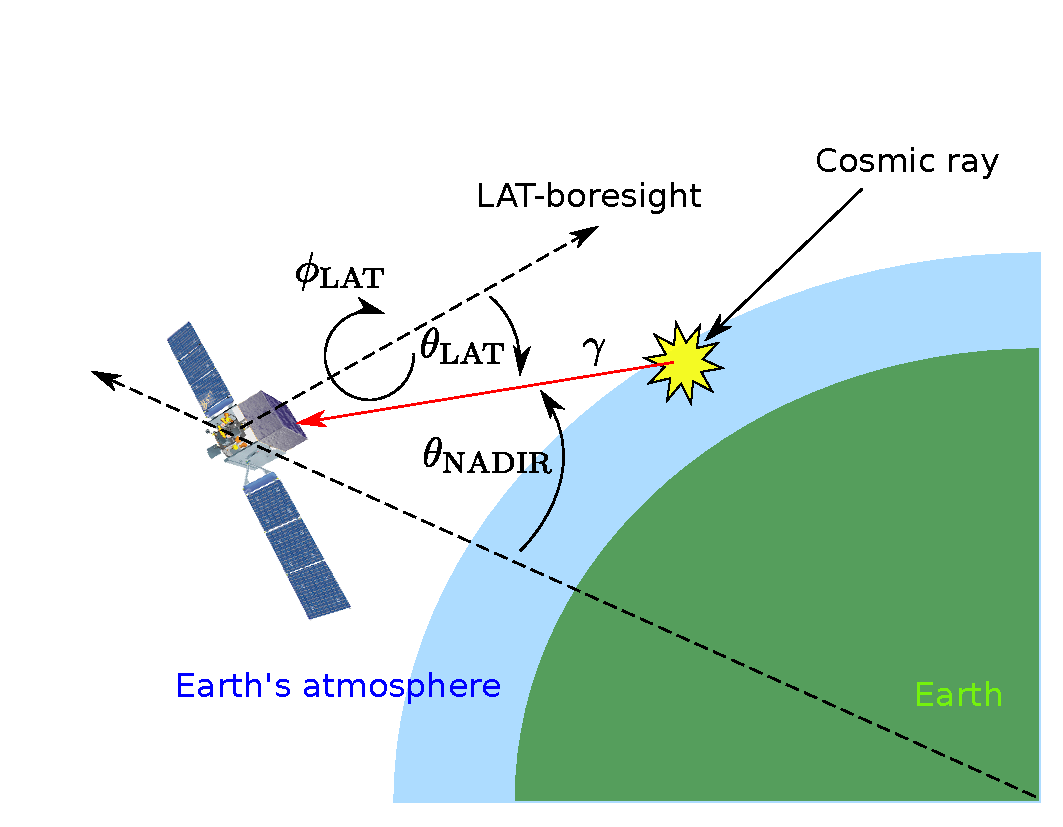
\includegraphics[width=0.5\textwidth]{img/gamma_production_schematic}
%     \caption{Schematic of $\gamma$-ray production}
%     \label{gamma_production_schematic}
% \end{figure}

% \begin{wrapfigure}{r}{0.5\textwidth}
%     \begin{center}
%         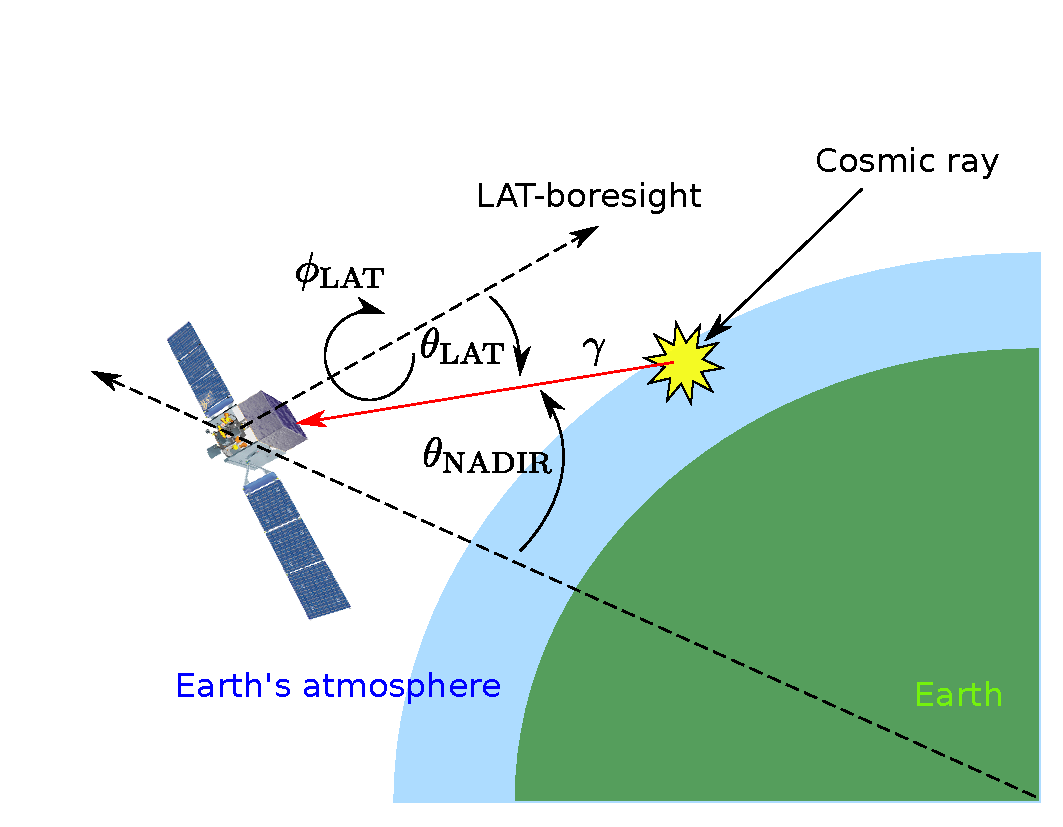
\includegraphics[width=0.5\textwidth]{img/gamma_production_schematic}
%     \end{center}
%     \caption{Schematic of $\gamma$-ray production}
%     \label{gamma_production_schematic}
% \end{wrapfigure}

\begin{figure}[h]
    \begin{minipage}{0.45\textwidth}
        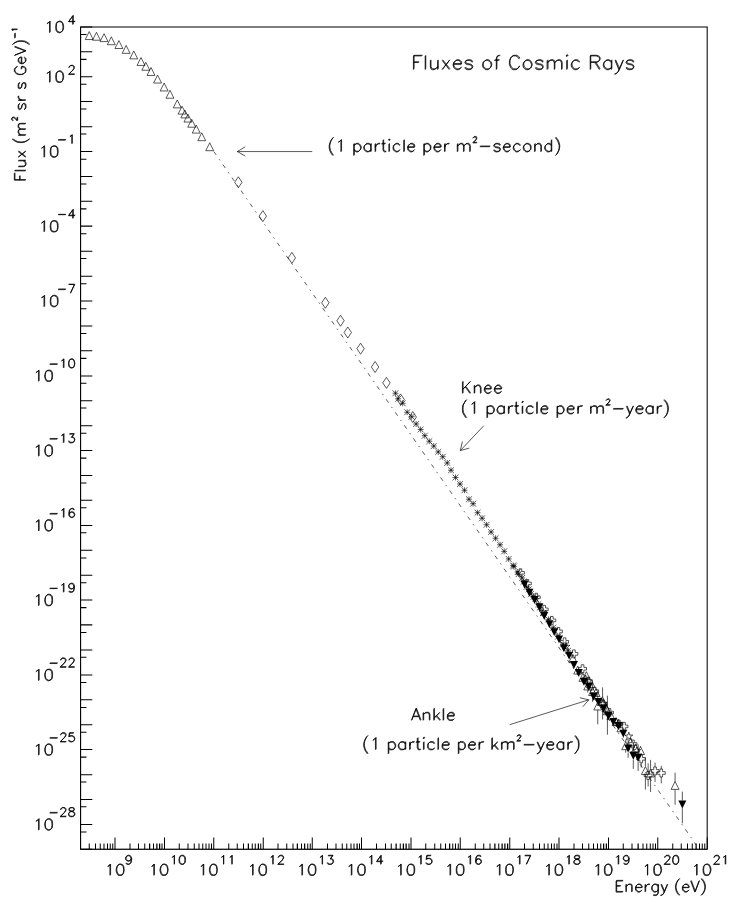
\includegraphics[width=\textwidth]{img/cr_knee_ankle}
        \caption{All-particle CR spectrum taken from \cite{Swordy2001}.}
        % \caption{The all particle spectrum of cosmic rays, image taken from }
        \label{cr_knee_ankle}
    \end{minipage}\hspace{2pc}
    \begin{minipage}{0.55\textwidth}
        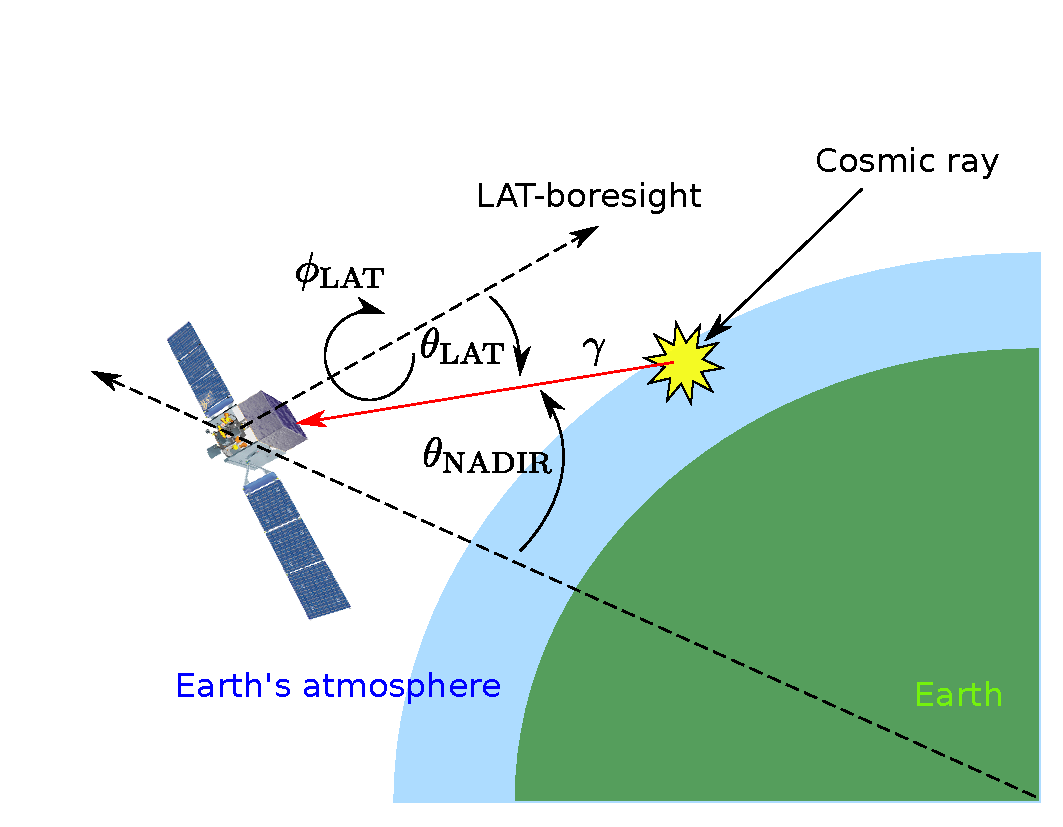
\includegraphics[width=\textwidth]{img/gamma_production_schematic}
        \caption{Schematic of high-energy Earth's $\gamma$-ray production}
        \label{gamma_production_schematic}
    \end{minipage} 
\end{figure}

% The observed flux is defined as differential flux where the governing equation
% for the calculation is represented as equation (\ref{flux_definition})
The observed flux for a given energy bin is calculated using
\begin{equation}
    \textbf{Flux} \equiv \frac{dN_\gamma}{dE} = \frac{\int_{\textrm{Limb region}}(\textrm{Count map}/\textrm{Exposure map})}{\Delta\Omega\Delta E }
    .\label{flux_definition}
\end{equation}

% Where count map is filled up with selected $\gamma$-ray and 
Here the count map is filled with numbers of photons, the exposure map represents 
the exposure time as well as the effective area of spacecraft 
which is a function of energy and $\theta_{\rm LAT}$, $\Delta E$ is the energy bin width,
and $\Delta\Omega$ is the solid angle of the thin-target Earth's limb region.
% Procedure of computation is begin with the requirement of 25 bins of histogram of
% the $\gamma$-ray flux which contain a various median of energy in each bin.
We perform the analysis with 25 bins of energy, equally spaced in logarithmic scale.
% Consequently, the number of count map and exposure map will be exactly the same as
% the energy bins. The calculation of exposure map is done by using log file of the
% spacecraft combine with the responsiveness of the spacecraft which has to be consider
% in every step time while spacecraft is online. 
For a given energy bin, the exposure map is calculated using the spacecraft's position
and orientation recorded in 30-second time steps, each of which involves a complex
coordinate transformation to create a map in the zenith-azimuth system.
Such computationally intensive task requires parallel
processing with Master-Slave technique that we have developed.
% which cause a huge amount of computing process.
% That is the reason why paralleling processing with Master-Slave technique is
% applied in this work.


\subsection{Interaction model}
In this work, we test 2 models of CR protons: single-power law (SPL) model
containing one spectral index, and broken-power law (SPL) model containing two
spectral indices with a break energy.

% The model for a scattering amplitude from hadronic collision \cite{K&Omodel}
% that could produce a photon as a secondary product which could be
% detected by \textit{Fermi}-LAT as equation \ref{eq:interaction_model}.
According to \cite{K&Omodel}, the secondary photon spectrum from proton-proton
collisions could be summarized by

\begin{equation}
    \frac{dN_\gamma}{dE_\gamma}\propto \int^{E_{\text{max}}}_{E_\gamma} dE'\frac{dN_p}{dE'} \frac{d\sigma^{pp\rightarrow\gamma}(E',E_\gamma)}{dE_\gamma}
    ,\label{eq:interaction_model}
\end{equation}

where here $dN_\gamma/dE_\gamma$ is the measured Earth's limb $\gamma$-ray spectrum,
$dN_p/dE'$ is the CR proton model, and $\sigma^{pp\rightarrow\gamma}$ is the interaction
cross section.
We take into account the contribution from CR He particles to the production of secondary
photons by using the cross section ratio ($\sigma_{\rm HeN}/\sigma_{p\rm N}$) from
\cite{WAtwater} and the He spectrum measurement by \cite{AMS-02Helium}. This modifies
Eq.~(\ref{eq:interaction_model}) to
% For the real use case, the interaction of an alphaparticle with the air
% has a significant contribution to the secondary photon.
% A modification of He-air interaction could be
% applied by using a fraction of cross-section from a given atomic number
% \cite{WAtwater}. The helium spectrum in rigidity is taken from the real
% measurement \cite{AMS-02Helium}. Then the input of the modified model
% is left only a proton spectrum.

\begin{equation}
    \frac{dN_{\gamma}}{dE_\gamma}(E_\gamma) \propto
    \sum_{E'_i}\left[\frac{E'_i}{E_{\gamma}}\Delta(\ln E'_i) \right]
    \left[ 
        f_{pp}\frac{dN_p}{dE'_i}
        \left\{
            1+\frac{\sigma_{\text{HeN}}}{\sigma{p\rm N}}\left(\frac{dN_p}{dR}\right)^{-1} \frac{dN_{\text{He}}}{dR} \frac{dR_{\text{He}}}{dR_p} 
        \right\}
    \right]
    ,\label{eq:derived_model}
\end{equation}

where $f_{pp} \equiv E_\gamma(d\sigma^{ij\rightarrow\gamma}/dE_\gamma)$
is the interaction cross section table in \cite{K&Omodel}.

\subsection{Optimization}

We use the SPL and BPL models for $dN_p/dE'$ in Eq.~(\ref{eq:derived_model}) and vary their parameters
(normalization, spectral indices, break energy) so that the resulting $dN_\gamma/dE_\gamma$
from the model fits to the measured Earth's limb $\gamma$-ray spectrum with maximum
likelihood. We employ the particle swarm optimization (PSO) \cite{pso_optimize} as our fitting algorithm
because PSO is efficient at avoiding local maxima and reaching the global maximum in
this multi-parameter problem.
% Optimizing a problem with multiple parameters might cause a local minimum
% which will cause an early stopping of the optimization proces before 
% reaching to the global minimum. In this work, a simple gradient optimization
% with a set of different initial values yield a various output which implicitly
% imply that there are local minimum exists in this problem. 
% To get rid of the local minimum, particle swarm optimization (PSO) is applied
% to find the best fit parameters \cite{pso_optimize}.





\section{Preliminary results}
The optimized parameters  for the SPL and BPL models are summarized in Table~\ref{tb:bestparams}. 
The best-fit $\gamma$-ray spectra from the two models
compared to the thin-target Earth's limb measurement by the LAT are illustrated
in figure~\ref{fig:gamma-flux}, showing very similar results for both models.
Since the proton-to-$\gamma$ energy conversion factor is roughly 0.17 for broad
and smooth spectra [10], our inferred CR proton spectra are valid between 60 - 2000 GV
in rigidity
% because the lower bound is a minimum rigidity of incoming proton that could produce a 10 GeV of $\gamma$-ray
% as shown in comparison with measurements by other instruments in Figure~\ref{fig:proton-flux}.
% Note that the normalizations of our work in Figure~\ref{fig:proton-flux} are scaled
% by fitting to AMS-02 data between 100~-~2000~GV.
because the lower bound is the mean rigidity of the incoming protons that produce 10-GeV $\gamma$ rays.
Our results are shown in comparison with measurements by other instruments in figure~\ref{fig:proton-flux}.
Note that the normalizations of our work in figure~\ref{fig:proton-flux} are scaled
by fitting to AMS-02 data between 100~-~2000~GV.

% eye to approximately match PAMELA data.
% has shown in Table~\ref{tb:bestparams}.
% According to figure \ref{fig:gamma-flux}, secondary $\gamma$-ray product
% from both SPL and BPL model yield a similar product via hadronic collision
% in the atmosphere. In order to validate the indirect measurement of CR proton,
% comparing with a real observations is mandatory which has shown
% in figure \ref{fig:proton-flux}. The normalization of this work is
% fitted PAMELA data to roughly scale the incident proton spectrum.

\begin{figure}[h!]
    \centering
    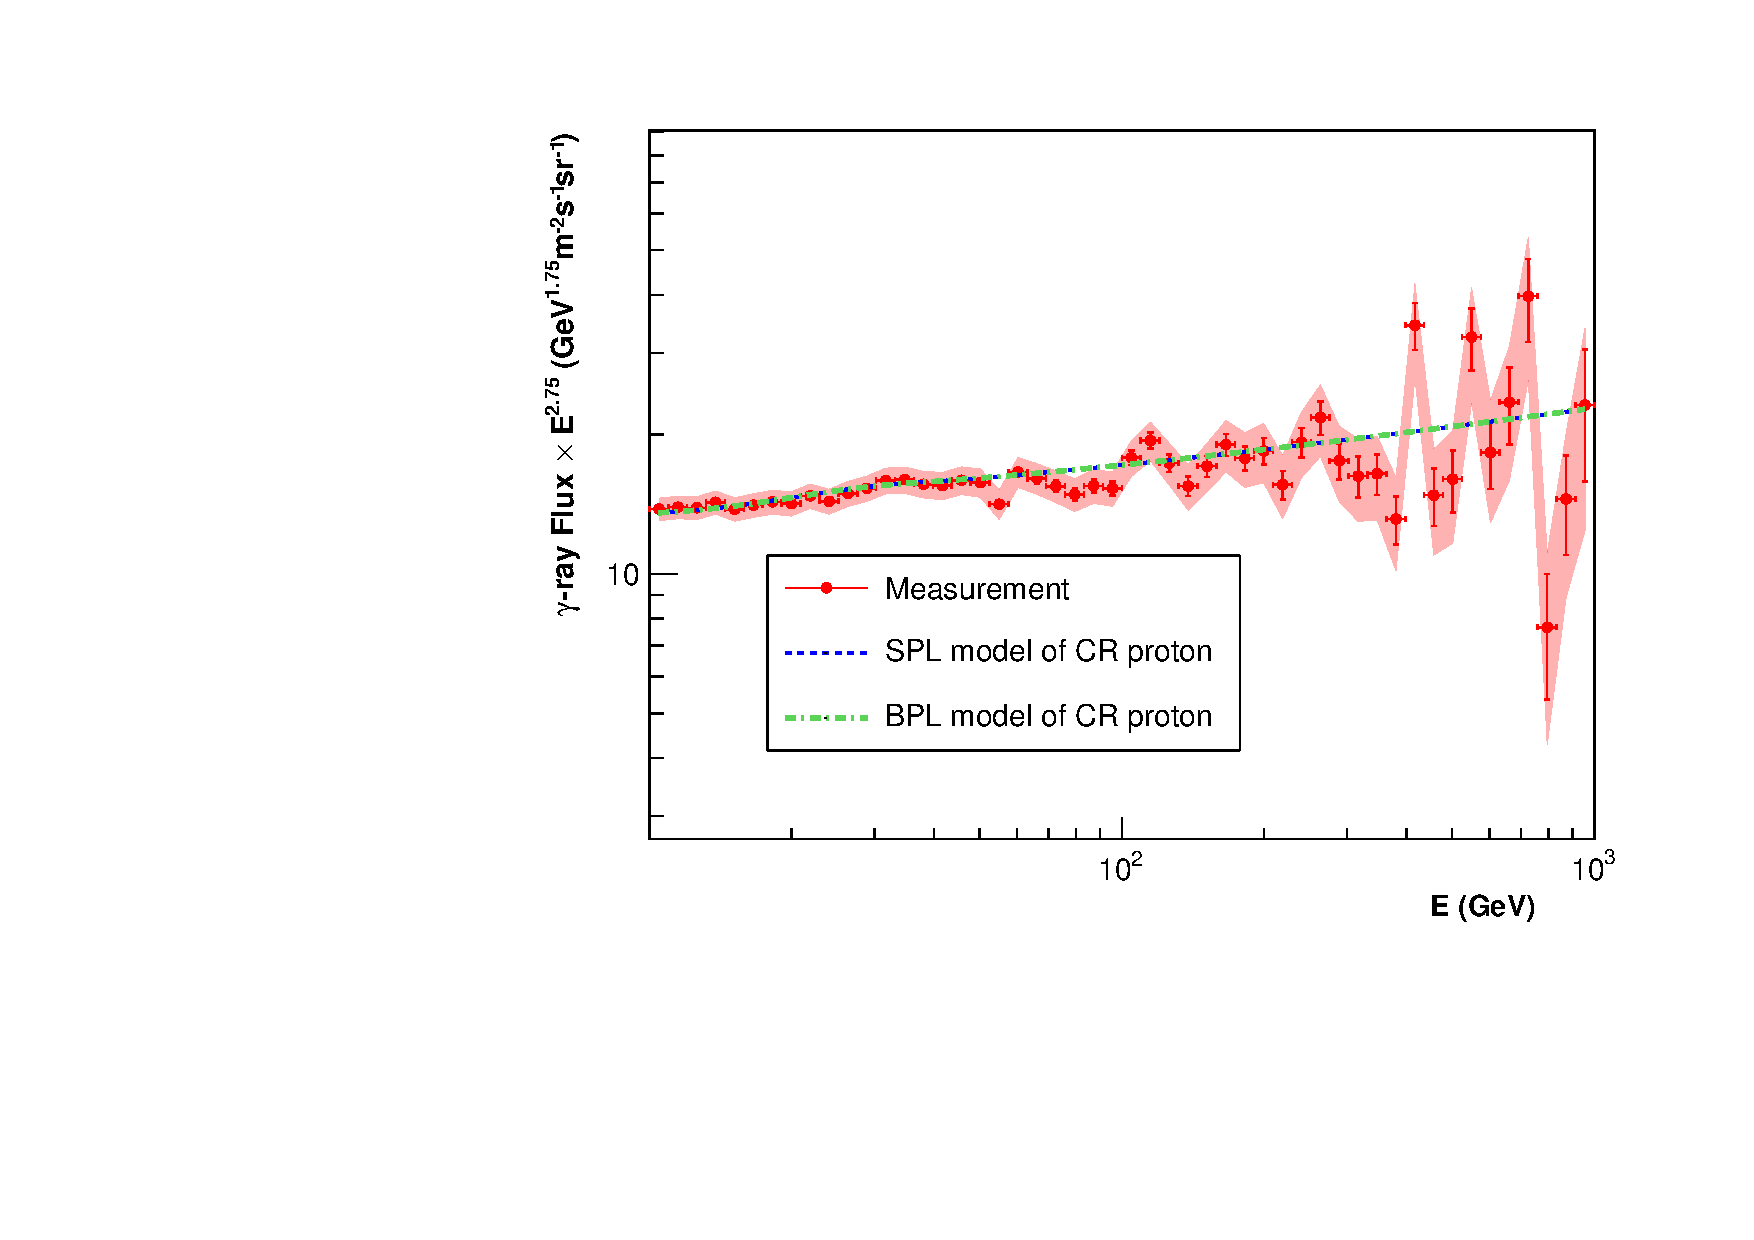
\includegraphics[width=0.7\textwidth]{img/fitted_result}
    % \caption{Measured $\gamma$-ray flux and the product from incident CRs}
    \caption{
        The $\gamma$-ray spectra calculated from the SPL (blue)
        and BPL (green) models of CR proton which best fit with the measured Earth's
        $\gamma$-ray spectrum in the thin-target regime (red).
    }
    \label{fig:gamma-flux}
\end{figure}



\begin{center}
\begin{table}[h]
\centering
\caption{Best-fit CR proton spectral parameters} 
\label{tb:bestparams}
\begin{tabular}{@{}l*{15}{l}}
\br
CR proton model&Index 1&Index 2&$E_\text{break}$ (GeV)\\
\mr
SPL&2.70&-&-\\
BPL&2.86&2.63&333\\
\br
\end{tabular}
\end{table}
\end{center}


\begin{figure}[h!]
    \centering
    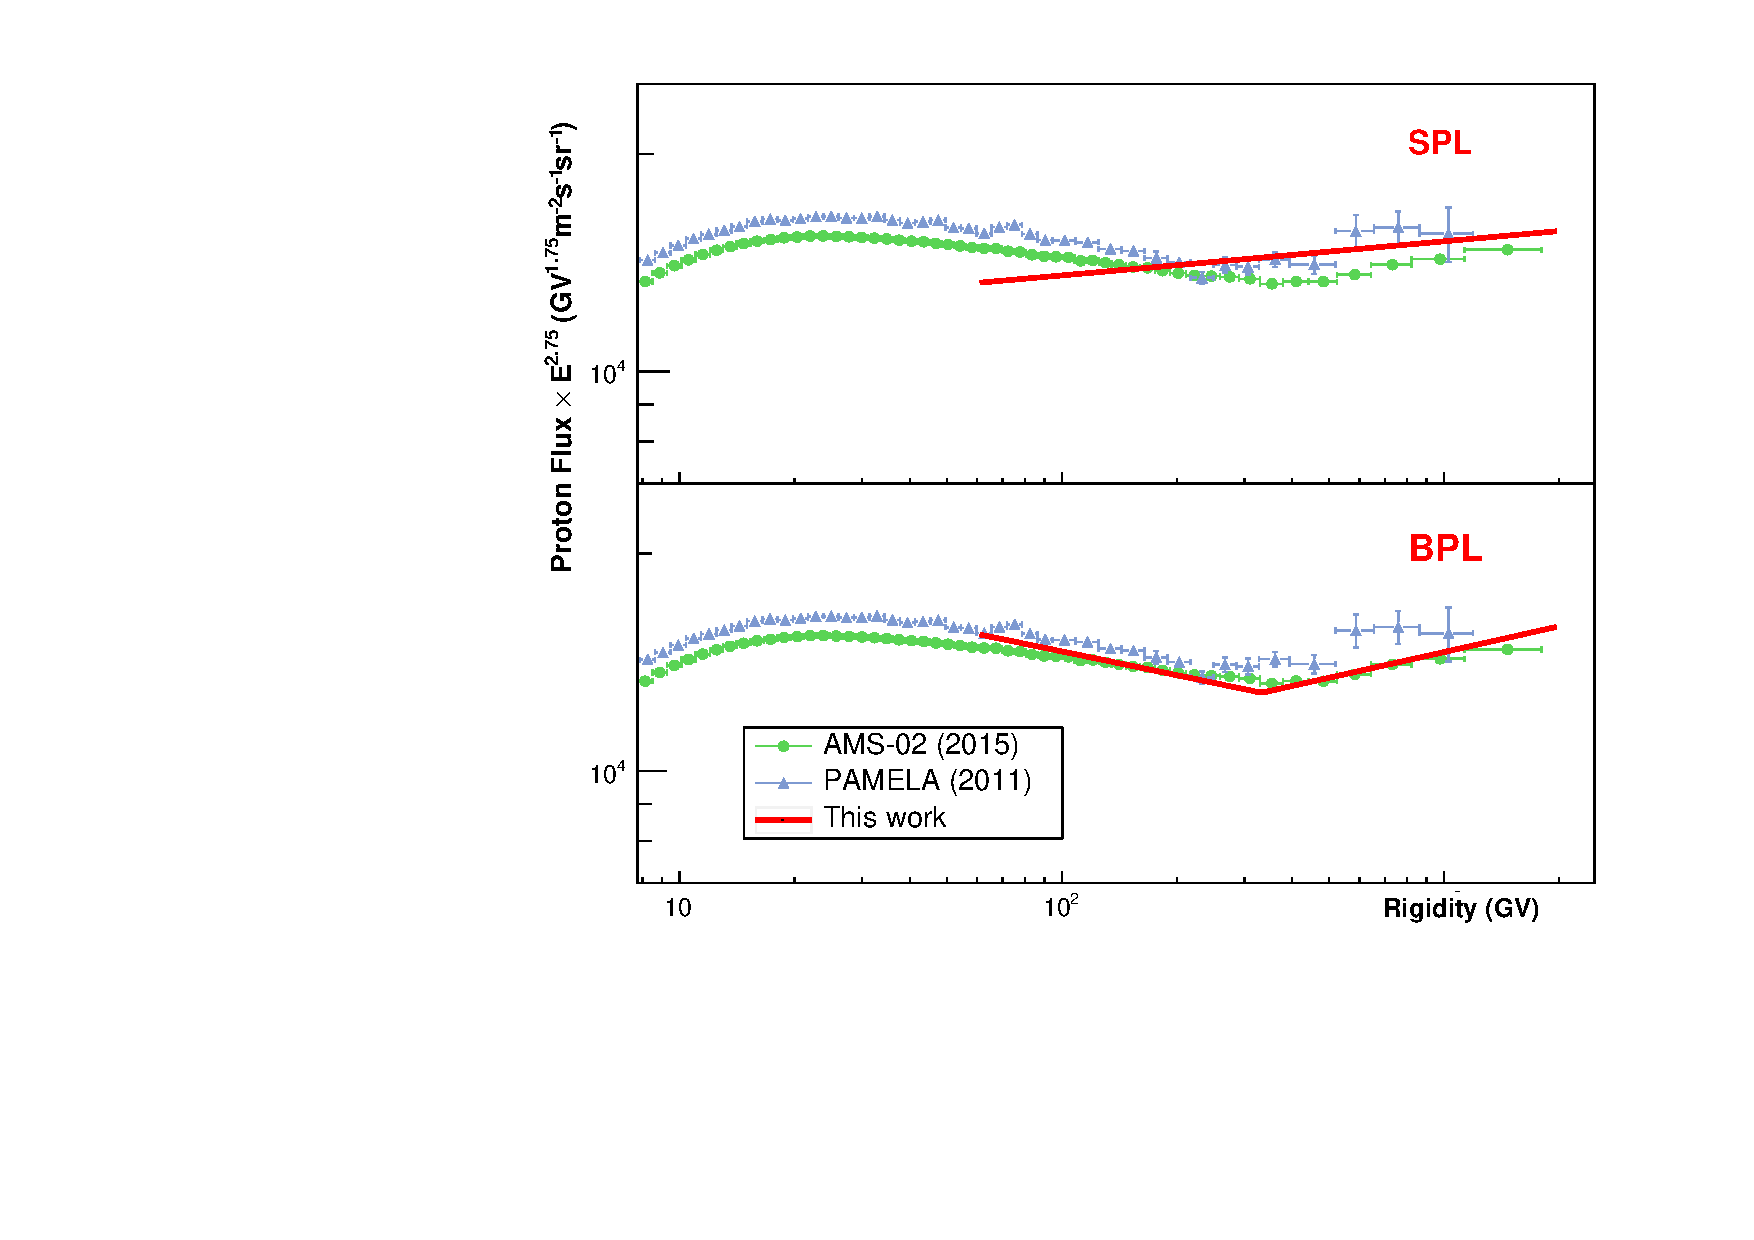
\includegraphics[width=0.8\textwidth]{img/ProtonSpectrumModelMeasurement.pdf}
    % \caption{Best fitted proton CRs versus real observations}
    \caption{Best-fit CR proton spectrum from this work (red) compared to the measurements by AMS-02 (blue) and PAMELA (green).}
    \label{fig:proton-flux}
\end{figure}



\section{Discussion and future work}
The best-fit BPL model of CR proton from this work are consistent with direct
measurements as shown in figure~\ref{fig:proton-flux}.
% The result also put weight on the previous study that we could take a
% benefit of brightness $\gamma$-ray from Earth's high atmosphere to indirectly observe cosmic
% ray spectrum which cause it’s luminosity.
We will need to determine whether the BPL model fits the data significantly better
than the SPL model does using likelihood ratio test to quantify the level of
confidence. We also plan to determine the statistical and total uncertainties of
the fit results by performing Monte Carlo simulations.
This work emphasizes that we could utilize the bright $\gamma$-ray emission
of the Earth's upper atmosphere to indirectly observe various properties of CRs.

\begin{figure}
    \centering
    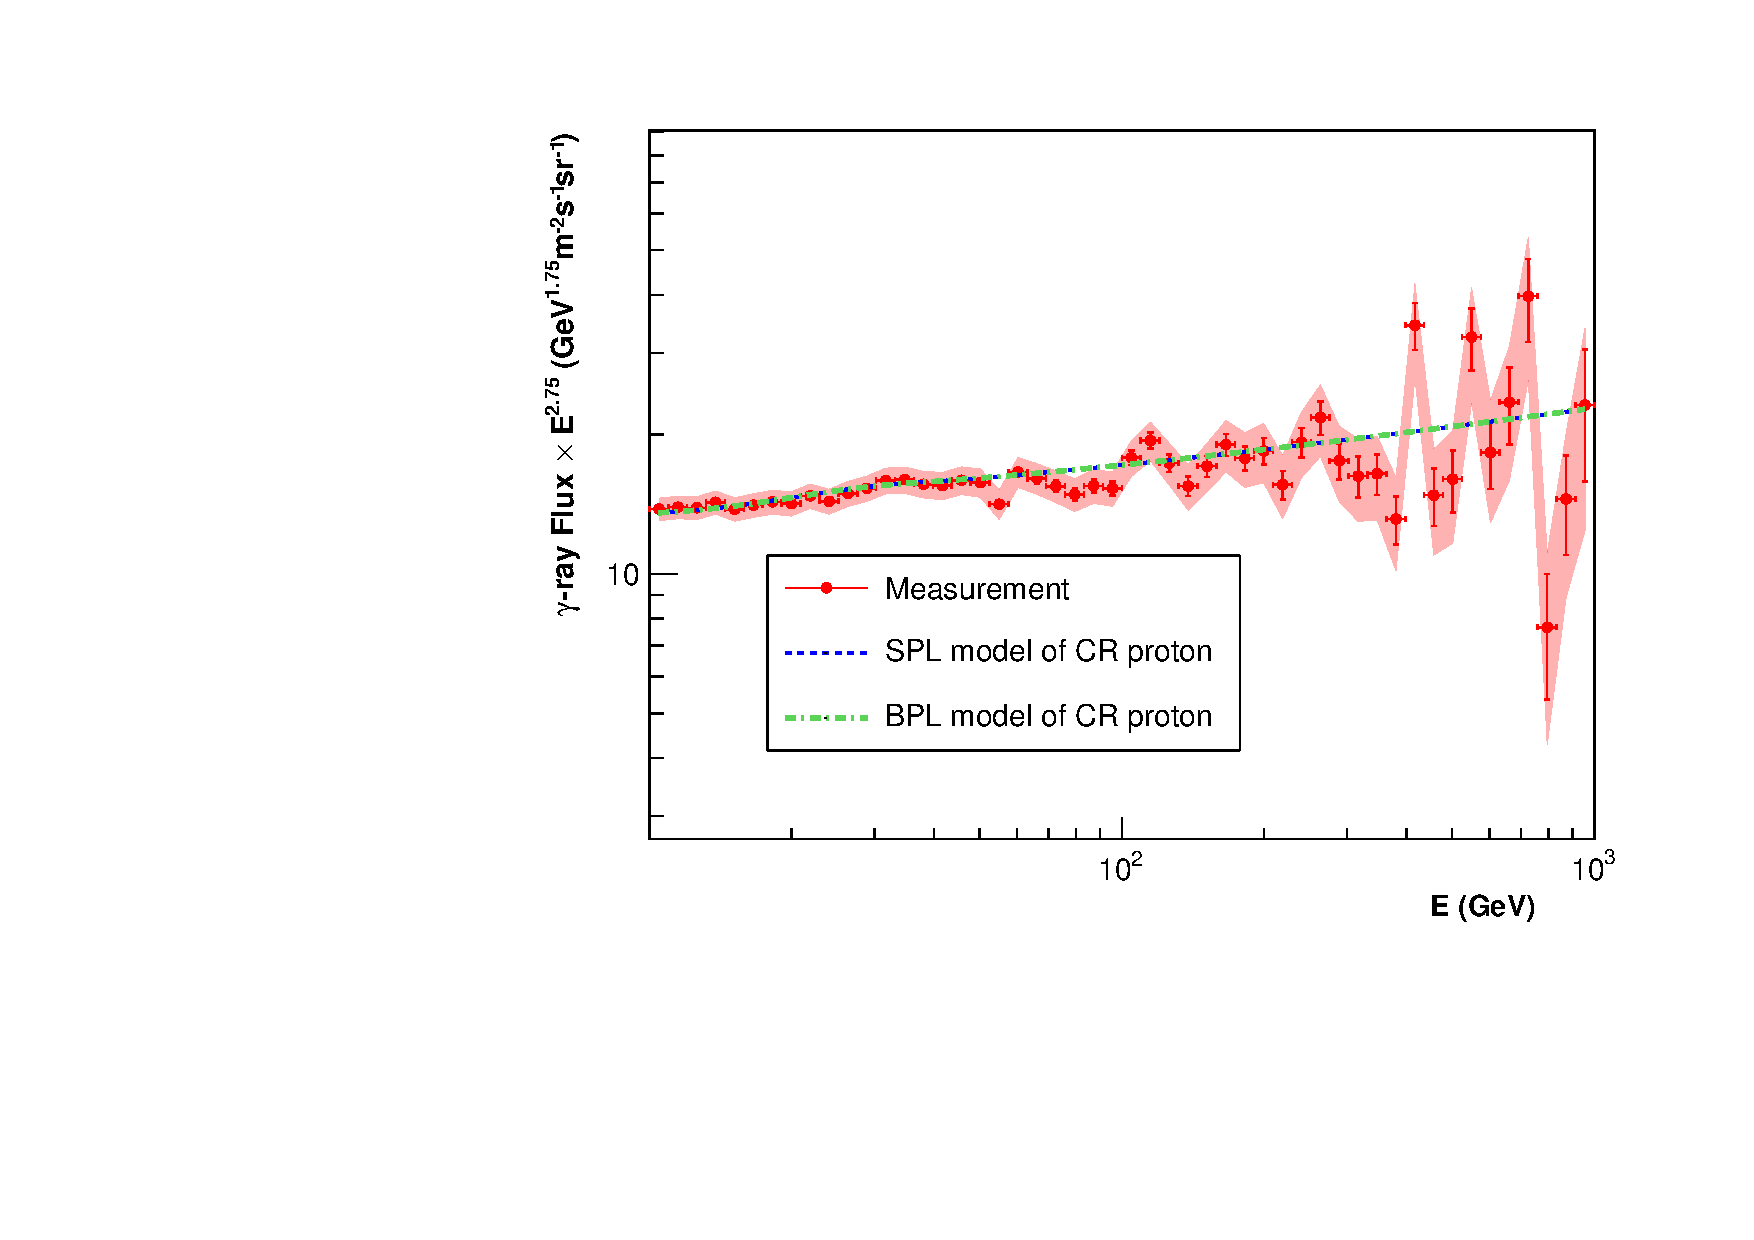
\includegraphics[width=0.8\textwidth]{img/fitted_result}
    % \caption{Measured $\gamma$-ray flux and the product from incident CRs}
    \caption{
        The $\gamma$-ray spectra calculated from the SPL (blue)
        and BPL (green) models of CR proton which best fit with the measured Earth's
        $\gamma$-ray spectrum in the thin-target regime (red).
    }
    \label{fig:gamma-flux}
\end{figure}


\begin{center}
\begin{table}
\centering
\caption{Best-fit CR proton spectral parameters.} 
\label{tb:bestparams}
\begin{tabular}{@{}l*{15}{l}}
\br
CR proton model&Index 1&Index 2&$E_\text{break}$ (GeV)\\
\mr
SPL&2.70&-&-\\
BPL&2.86&2.63&333\\
\br
\end{tabular}
\end{table}
\end{center}


\begin{figure}
    \centering
    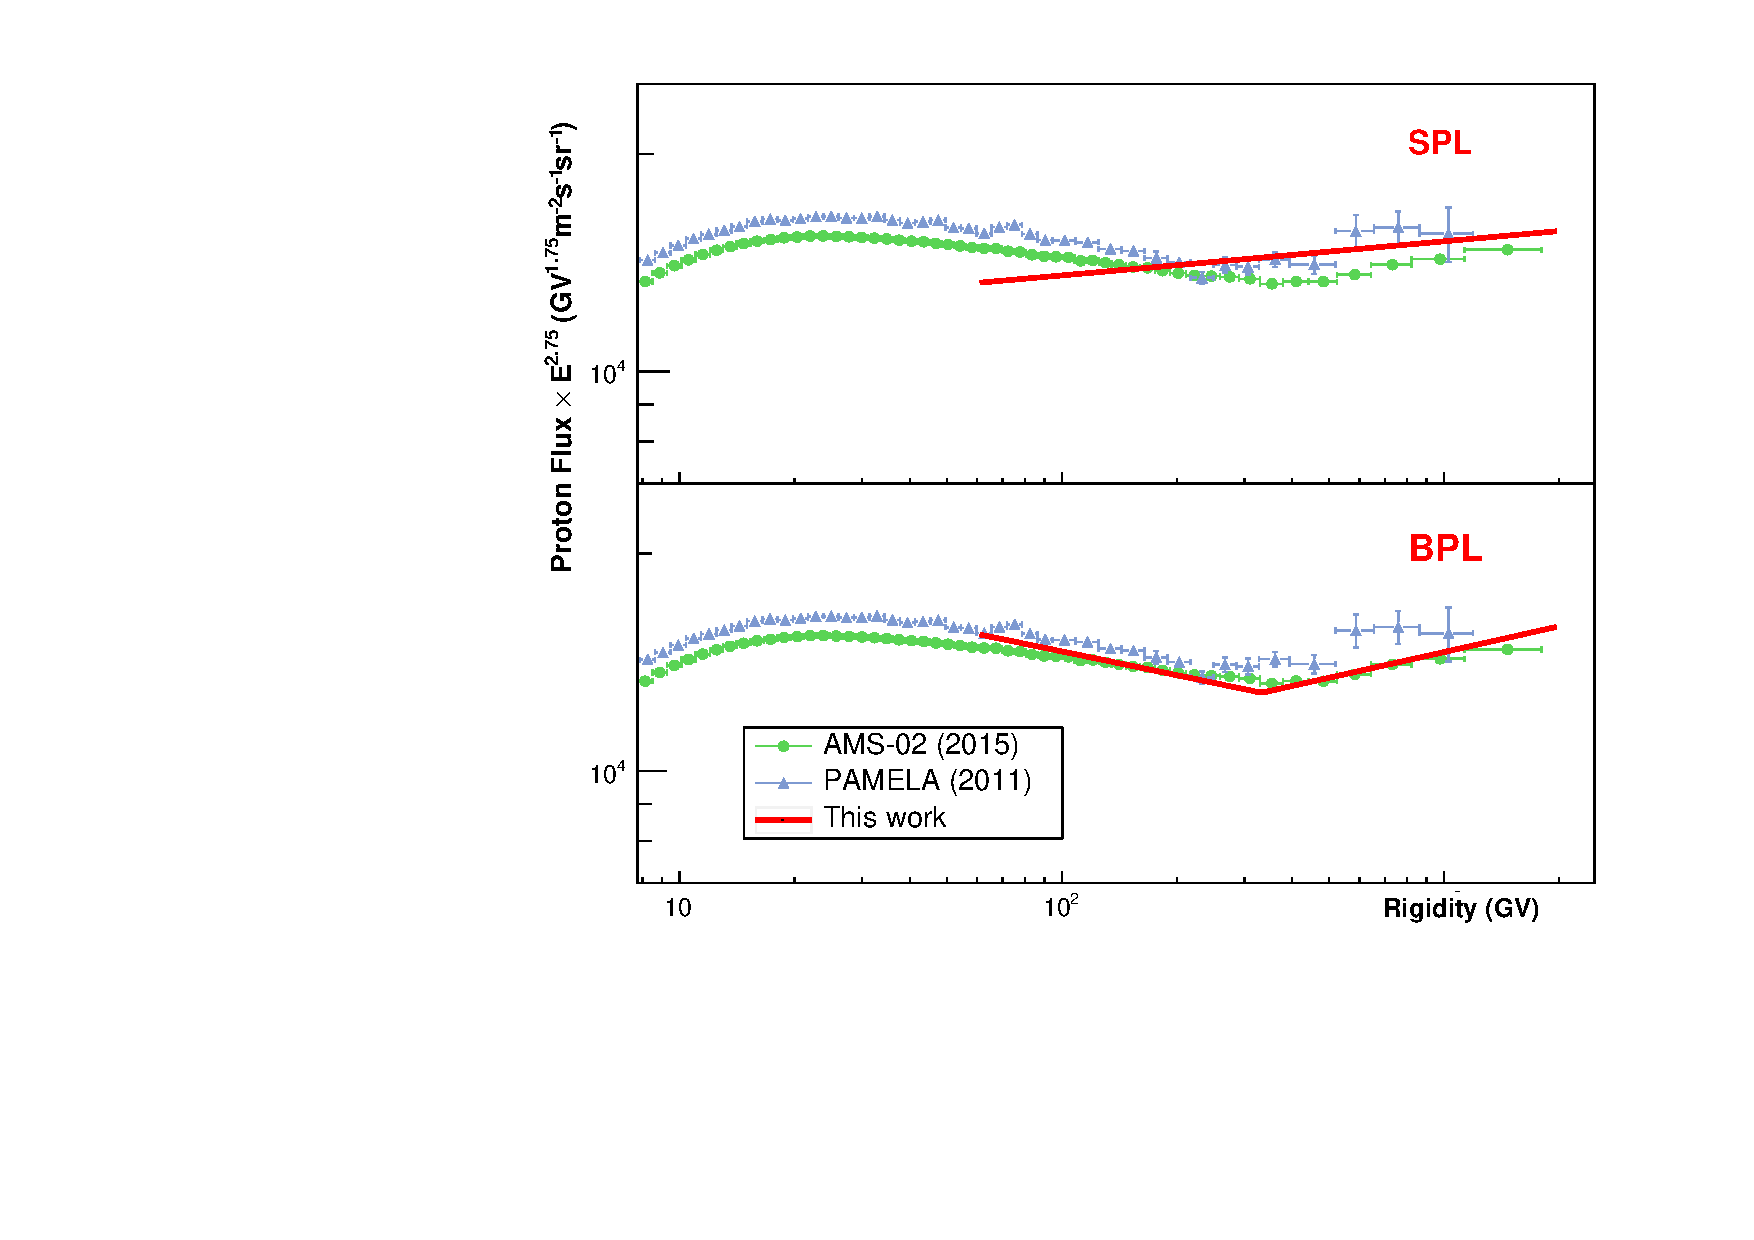
\includegraphics[width=0.9\textwidth]{img/ProtonSpectrumModelMeasurement.pdf}
    % \caption{Best fitted proton CRs versus real observations}
    \caption{Best-fit CR proton spectrum from this work (red) compared to the measurements by AMS-02 (blue) and PAMELA (green).}
    \label{fig:proton-flux}
\end{figure}

% From Figure~\ref{fig:gamma-flux}, a trend of incident proton model
% demonstrated that BPL has more consistency than SPL. Nevertheless,
% to determine the significance between two models require likelihood
% ratio test to evaluate the statistical level of confidence. In addition,
% statistical and total error including the instrument will be determined
% by performing Monte Carlo Simulation.






\section*{Acknowledgments}
\par I would like to express my deep gratitude to 
Assist.~Prof.~Warit~Mitthumsiri and Prof.~David~Ruffolo for their patient guidance.
I would also like to thank people at the space physics laboratory at Mahidol University
for their support.
This research project is partially supported by Thailand Science Research
and Innovation (RTA6280002).

\FloatBarrier

\section*{References}
% \bibliographystyle{abbrv}
\bibliographystyle{iopart-num}
% \bibliographystyle{unsrt}
\bibliography{iopart-num_short}

\end{document}


